% !TeX program = xelatex
% !TeX root = main.tex
\begin{frame}[label=pc-why]{同一投资者的研究主题如何共同出现}
  \crumb{Part 4}{4.1 股票与投资者 · 投资者层}{VI · Table 5}
  \pair{\textbf{股票月回答}\par\small
    什么股票和主题被常看？\par
    是股票-月份的 panel，\(Y\) 是覆盖、用时。}
  {\textbf{投资者（家庭）层回答}\par\small
    同一个人会一起看哪些主题？这些模式和他关注股票的类型是否共变？}
  \medskip
  \leadrow{交易频率不太有用}{因为交易笔数与每笔研究分钟的 Pearson 相关为 \(-0.10\)，秩相关为 \(-0.22\)。}
  \finding{在投资者层，用 PCA（主成分分析模型）概括主题参与、股票倾向的主要变异方向。}
\end{frame}

\begin{frame}[t,label=pc-input]{PCA 输入：主题参与与投机标的倾向}
  \crumb{Part 4}{4.1 股票与投资者 · 输入矩阵}{VI · Table 5}
  \vspace{-.65em}
  \setlength{\abovedisplayskip}{3pt}
  \setlength{\belowdisplayskip}{4pt}
  \[
    B_{ik}=\mathbf{1}\{m_{ik}>2\},
    \qquad X_i=(B_{i1},\ldots,B_{i,13},S_i),
    \qquad R=\frac{Z^\top Z}{n-1}.
  \]
  \small
  \setlength{\parskip}{1pt}
  \renewcommand{\arraystretch}{1.06}
  \textbf{输入格式例子}\par\smallskip
  \begin{tabularx}{\linewidth}{@{}l*{4}{Y}L{.21\linewidth}@{}}
    \toprule 投资者 & 价格图 & 盈利 & 分析师 & \(\cdots\) & 投机标的倾向\\\midrule
    A & 1 & 0 & 1 & \(\cdots\) & \(S_A\)（连续）\\
    B & 1 & 1 & 0 & \(\cdots\) & \(S_B\)（连续）\\
    C & 0 & 1 & 1 & \(\cdots\) & \(S_C\)（连续）\\\bottomrule
  \end{tabularx}\par\smallskip
  \(m_{ik}\) 为该户在该主题的月均研究分钟。\textbf{严格大于 2 分钟记 1，否则记 0。}\par
  实际输入为 13 个主题指标和连续的 \(S_i\)。\(S_i\) 高偏小、新、高波动股，低偏大、成熟、分红股。\par
  \(Z\) 为按列标准化的输入矩阵，\(n\) 为投资者数。\(R\) 的特征向量给出主成分方向。
\end{frame}

\newcommand{\loadingbar}[4]{%
  \node[anchor=east,inner sep=2pt] at (-.58,#1) {#2};
  \fill[#4!75] (0,#1-.18) rectangle (#3,#1+.18);
  \node[anchor=west,inner sep=2pt] at ({max(0,#3)},#1) {\pgfmathprintnumber[fixed,precision=2]{#3}};}
\begin{frame}[label=pc-one]{第一主成分刻画跨主题的共同参与}
  \crumb{Part 4}{4.1 股票与投资者 · PC1}{Table 5}
  \begin{columns}[T,onlytextwidth]
    \column{.63\textwidth}\centering
    \begin{tikzpicture}[x=6.7cm,y=.55cm,font=\small]
      \begin{scope}[xshift=2.3cm]
      \node[anchor=east,inner sep=2pt] at (0,6) {主题或股票倾向};
      \draw[quiet!30] (0,-.30)--(0,5.35);
      \foreach \y/\name/\v in {5/{未知新闻}/.36,4/{快照}/.32,3/{分析师}/.32,2/{价格图}/.31,1/{盈利}/.29,0/{投机标的倾向}/.01}{
        \node[anchor=east] at (0,\y) {\name};
        \fill[sampleblue!70] (0,\y-.17) rectangle (\v,\y+.17);
        \node[anchor=west] at (\v,\y) {\pgfmathprintnumber[fixed,precision=2]{\v}};}
      \end{scope}
    \end{tikzpicture}\par
    \column{.35\textwidth}
    \greatnum{26.81\%}\par
    {\small 解释输入总变异\\特征值 3.75}\par\medskip
    {\small 发现 13 项主题的载荷均为正，股票投机倾向近零。}
  \end{columns}
  \finding{第一主成分 PC1 被命名为研究强度：得分较高的投资者通常参与更多主题。}
\end{frame}

\begin{frame}[label=pc-two]{第二主成分把快信息与投机标的联系起来}
  \crumb{Part 4}{4.1 股票与投资者 · PC2}{Table 5}
  \begin{columns}[T,onlytextwidth]
    \column{.67\textwidth}\centering
    \begin{tikzpicture}[x=4.6cm,y=.41cm,font=\scriptsize]
      \draw[quiet!55] (0,-.36)--(0,8.36);
      \loadingbar{8}{留言板}{.46}{wine}
      \loadingbar{7}{投机标的}{.43}{wine}
      \loadingbar{6}{综合快照}{.30}{wine}
      \loadingbar{5}{价格图}{.19}{wine}
      \loadingbar{4}{分析师}{0}{quiet}
      \loadingbar{3}{技术信号}{-.11}{sampleteal}
      \loadingbar{2}{其他基本面}{-.29}{sampleteal}
      \loadingbar{1}{盈利}{-.34}{sampleteal}
      \loadingbar{0}{股利}{-.47}{sampleteal}
    \end{tikzpicture}\par
    \column{.31\textwidth}
    \greatnum{8.77\%}\par
    {\small 解释输入总变异\\特征值 1.23}\par\medskip
    {\small 研究快信息与偏向投机标的在同一轴上。盈利、股利靠相反一侧。}
  \end{columns}
  \finding{第二主成分 PC2，作者猜测命名为投机性偏好。}
\end{frame}

\subsection{4.2 交易时点与路径}
\begin{frame}[label=timing]{投资者在同股交易前的研究时间}
  \crumb{Part 4}{4.2 交易时点与路径 · 研究何时发生}{Figure 3 · 50 户}
  \pair{\centering\small\textbf{均值}\par
    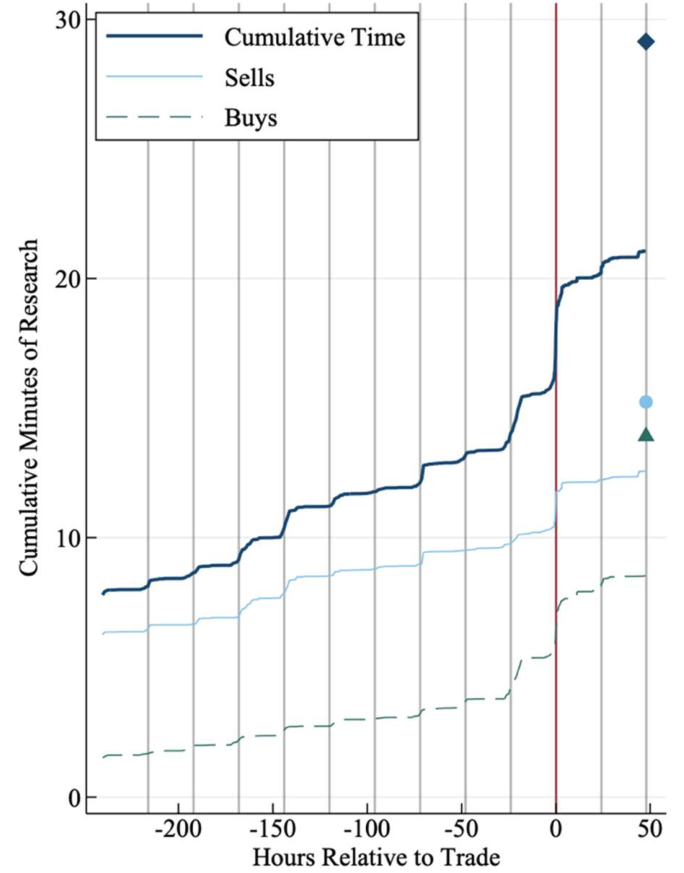
\includegraphics[width=\linewidth,height=4.04cm,keepaspectratio]{fig3-mean-plot.png}\par}
  {\centering\small\textbf{中位数}\par
    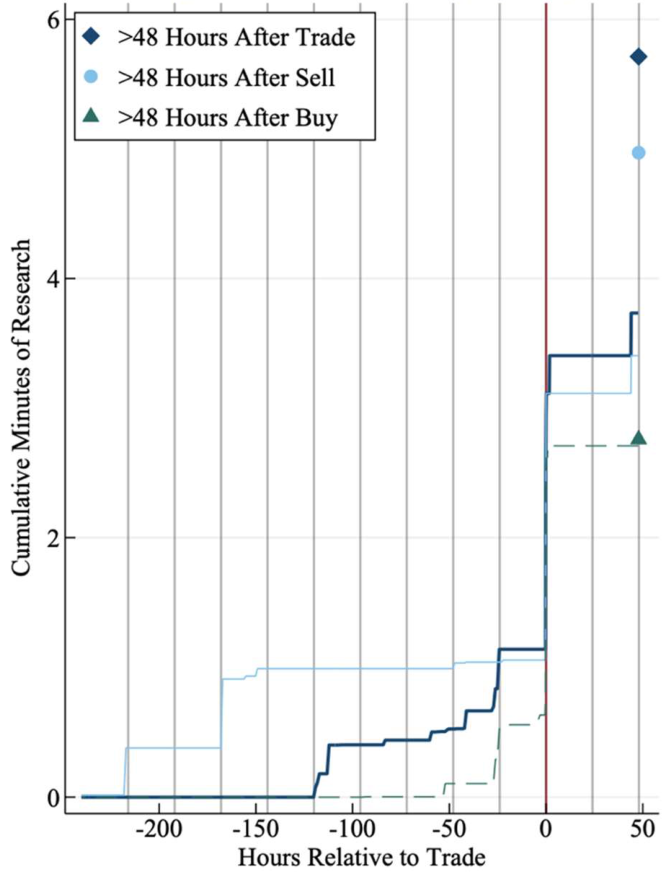
\includegraphics[width=\linewidth,height=4.04cm,keepaspectratio]{fig3-median-plot.png}\par}
  {\small 横轴：距本次交易的小时，\(0\) 为订单。纵轴：累计研究分钟。}
  \finding{约到交易前五天才见中位数累积，主要跳升临近下单；均值在更早时点也有累积。}
\end{frame}

\begin{frame}[label=path]{新的同股路径常在首个主题后结束}
  \crumb{Part 4}{4.2 交易时点与路径 · 主题之间的跳转}{Figure 4}
  \begin{columns}[T,onlytextwidth]
    \column{.61\textwidth}\centering
    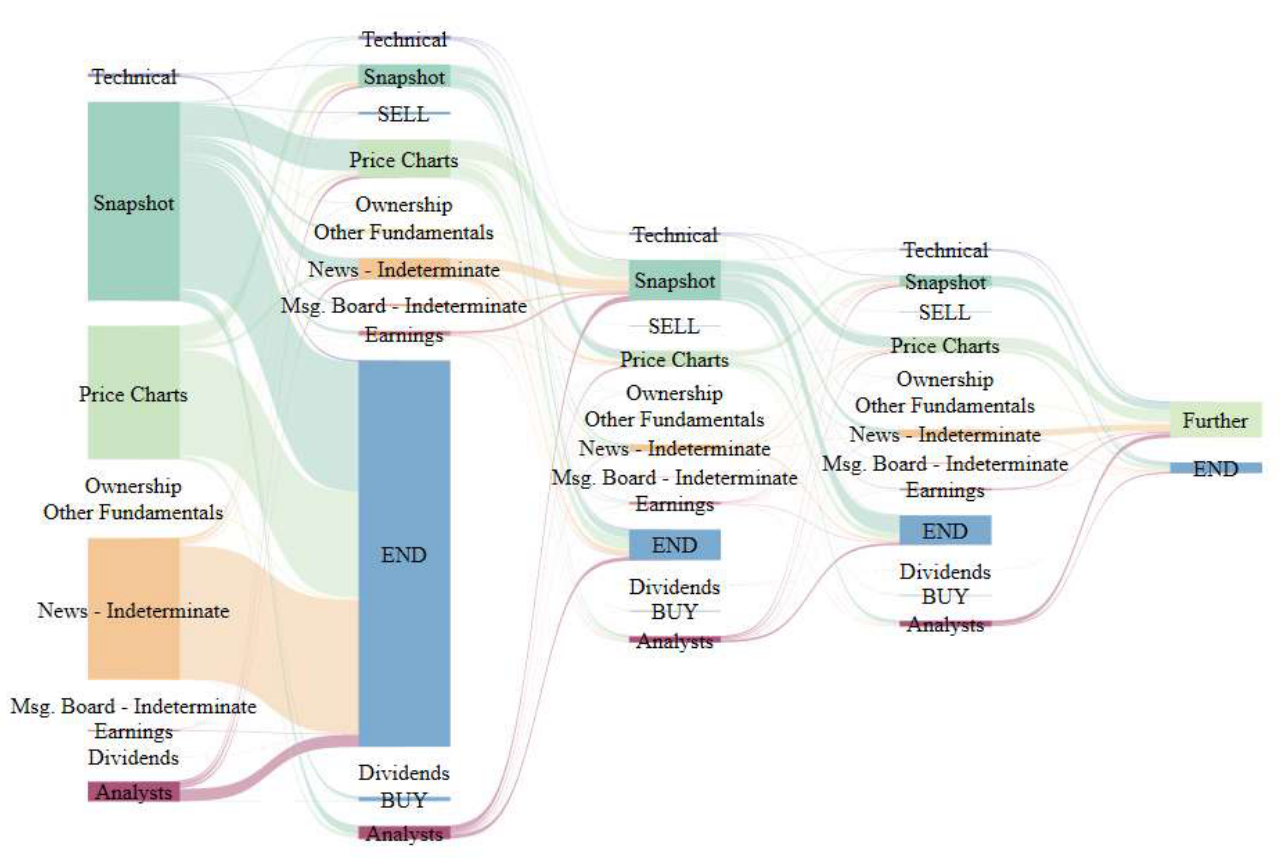
\includegraphics[width=\linewidth,height=4.6cm,keepaspectratio]{fig4-plot.png}
    \column{.36\textwidth}\small
    \leadrow{入口}{快照、价格图、新闻较常见。}
    \leadrow{第二列 END}{最粗一支，表示首个主题后没有新增的计入主题。}
    \leadrow{右端 Further}{仍有更多出现的主题。}
    \medskip
    线宽为路径数。
  \end{columns}
  \finding{例：价格图 \(\to\) 盈利 \(\to\) 再看价格图，图上只留价格图 \(\to\) 盈利。484 户，16,930 个同股十天窗口。}
\end{frame}

\begin{frame}[label=fast-slow]{按研究风格分组后，快信息组路径更窄}
  \crumb{Part 4}{4.2 交易时点与路径 · 按 PC2 分组}{Figure 5 C/D}
  \pair{\centering\small\textbf{C · 慢信息，PC2 最低五分位}\par
    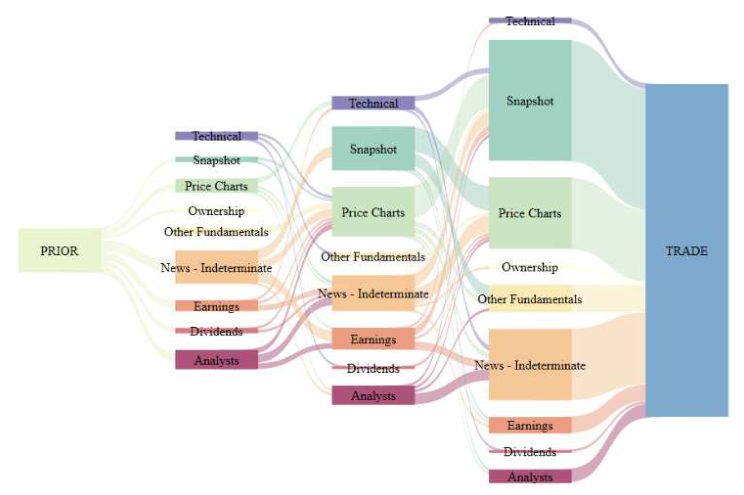
\includegraphics[width=\linewidth,height=3.68cm,keepaspectratio]{fig5c-plot.png}\par}
  {\centering\small\textbf{D · 快信息，PC2 最高五分位}\par
    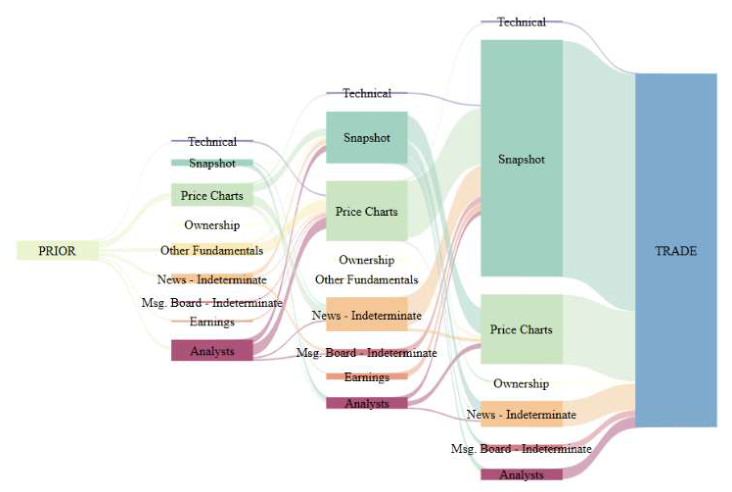
\includegraphics[width=\linewidth,height=3.68cm,keepaspectratio]{fig5d-plot.png}\par}
  {\small 按投资者得分 \(\mathrm{score}_{i,2}=z_i^\top v_2\) 取最低和最高五分位。
  \(z_i\) 为该投资者的标准化输入，\(v_2\) 为 PC2 方向。}\par\smallskip
  {\small 慢信息组路径更宽；快信息组，一般在快照和价格图中多出现。线宽为路径数。}
\end{frame}
